\section{Evaluation}
\label{sec:evaluation}

We evaluate \name{} on the Waymo and Cityscapes data. %The highlights are:

\begin{itemize}
    \item With multiple cameras sharing the resources on an edge server, \name{} achieves upto \romilc{16}\% \romil{This is sim, check exact with zhengxu} points higher accuracy than the fair sharing baseline. Attaining the same accuracy with a fair-sharing scheduler would require upto \romilc{$2.xx\times$} more resources.
    \item With the same resource provisioning, \name{} is able to support upto $5\times$ more video streams than the fair scheduler.
    \item \name{}'s performance gracefully degrades with reduction in resources to the baseline that does not retrain since it evaluates the cost of retraining on the accuracy. 
\end{itemize}

\subsection{Methodology}
\label{subsec:eval-setup}

\junchen{need to update}

\noindent\textbf{Datasets.} For our evaluation, we use the Waymo Open\cite{waymo} and Cityscapes\cite{cityscapes} datasets, two popular video datasets containing dashboard camera footage of cars driving through cities in the US and Europe. Cityscapes has frames from 27 video streams training with a total of 5000 pixel-level annotated frames, while Waymo Open has 1000 video segments with a total of 200000 frames.

The workload in Cityscapes is constructed by treating each city's video as an independent video stream feeding into {\name} for inference and retraining. The workload in Waymo Open is constructed by creating video streams by concatenating 20s-video segments belonging to the same city in chronological order. Each video stream in both datasets is then split into 10 retraining windows. These workloads are representative of independent video-streams with local variations which necessitate retraining for their specific data-distributions.



% \noindent\textbf{System Implementation.}\junchen{shrink or remove given the impl section}
% We implement a prototype of \name in Python using Ray\cite{ray} for asynchronous operations and RPCs. 
% Each video stream is modelled as an independent Ray actor whose resource allocation for inference and training is periodically updated by the Ekya master.

% % Write about microprofiling
% %\mypara{Microprofiling}
% The Ekya implementation ingests video streams and splits it into evenly sized retraining periods. At the start of each retraining period, the hyperparameters are micro-profiled \ref{sec:microprofiling} and the thief scheduler is run to compute the resource allocations for training and inference jobs. 
% %This resource allocation is then enforced by Ekya by launching new training processes and restarting the inference processes with updated resource weights. 

% Ekya requires fine-grained GPU allocation between inference and training processes. 
% Talk about memory isolation in Ekya.
% Talk about nvidia MPS resource sharing



\noindent\textbf{Trace driven simulator.}
% \junchen{update this?}
In addition to the system implementation \cref{sec:system}, we also built a simulator to simulate the execution of training and inference jobs under varying resource constraints and workloads. The inputs to the simulator are execution traces from training and inference workloads with different configurations. 

To collect execution traces, we ran all configurations in our hyperparameter space on the 10 retraining windows for every video stream in the Waymo and Cityscapes datasets. For each training job execution in a retraining window, we log the training-accuracy progression over GPU-time. Once the model is trained, we also log its test accuracy over the future retraining windows to get the accuracy in future windows if it was not retrained. This builds an exhaustive trace set that allows us to simulate custom scheduling policies, modify the execution order, simulate resource sharing and allocation. All profiling and trace collection was done on a testbed with Nvidia RTX 2080 and Intel Xeon E-2226G CPU.

% Talk about the assumptions - inference accuracy min GPU, linear scaling etc

\textbf{Hyperparameters.}
For each training job, we create a fixed set of configurations by varying the following hyperparameters - number of epochs to train, batch size, number of neurons in the last layer, number of layers to retrain, and the fraction of data between retraining windows to be used for retraining. We then selected combinations of these hyperparameters to create a diversity in the resource-accuracy profiles of the configurations. 

\mypara{Performance metrics}
\junchen{tbd: accuracy, throughput (\# of streams) under given \# of gpus}

\textbf{Baselines.}
We compare the thief scheduler against a weighted {Fair Scheduler} \cite{fair-1, fair-2, videostorm}, which allocates equal resources to all video streams and within a video stream, allocates resources to training and inference proportional to the weight set as the \lstinline{inference_weight} parameter to scheduler. A higher \lstinline{inference_weight} implies a higher resource allocation to inference and a reduced allocation to training jobs. To pick retraining hyperparameters, the fair scheduler employs the common heuristic of highest-accuracy first. 

%We compare against two baselines. First is \textit{No-retraining}, which does not ever retrain the model and thus allocates resources only to inference. Second is \textit{Fair Scheduler} \cite{fair-1, fair-2, videostorm} which allocates equal resources to all video streams and within a video stream, allocates equal resources to both, training and inference. To pick retraining hyperparameters, the fair scheduler employs the common heuristic of highest-accuracy first. 
% Why are these good baselines?

% \textbf{Metrics.}
% % More:
% Our most used metric is Inference Accuracy over time, as described in \S\ref{subsec:formulation}. We also use the number of GPUs provisioned at the edge server as a measure of cost.


% \junchen{

% 6.2 Overall improvement

% - accuracy vs. gpus (fix \# of videos)

% - streams vs. gpus (fix accuracy)

% - accuracy vs. streams (fix \# of gpus)

% - alternative architectures



% 6.3 Understanding Ekya improvements

% - ablation analysis

% - per-stream gains

% - temporal behaviors



% 6.4 Microbenchmarking

% - estimation accuracy of microprofiling

% - impact of microprofiling erros

% - delay of thief scheduler

% - impact of scheduling granularity


% }

% overall improvement: 
% acc vs gpu
% mention the cloud baseline
\subsection{Overall improvements}

\begin{figure}
  \centering
%   \begin{subfigure}[t]{0.5\linewidth}
%     \centering
%     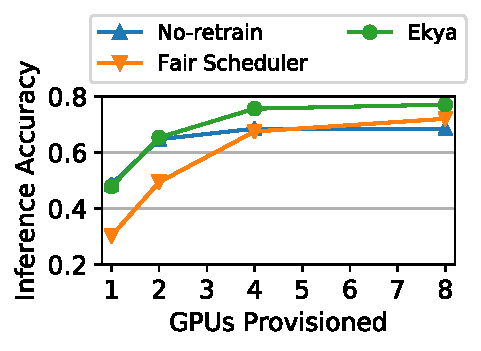
\includegraphics[width=\linewidth]{results/multicam/multicam_acc_vs_res_cityscapes.pdf} 
%     \caption{Cityscapes}
%     \label{fig:scalability-gpus-cityscapes}
%   \end{subfigure}
%   ~~~
%   \begin{subfigure}[t]{0.5\linewidth}
%     \centering
%     % 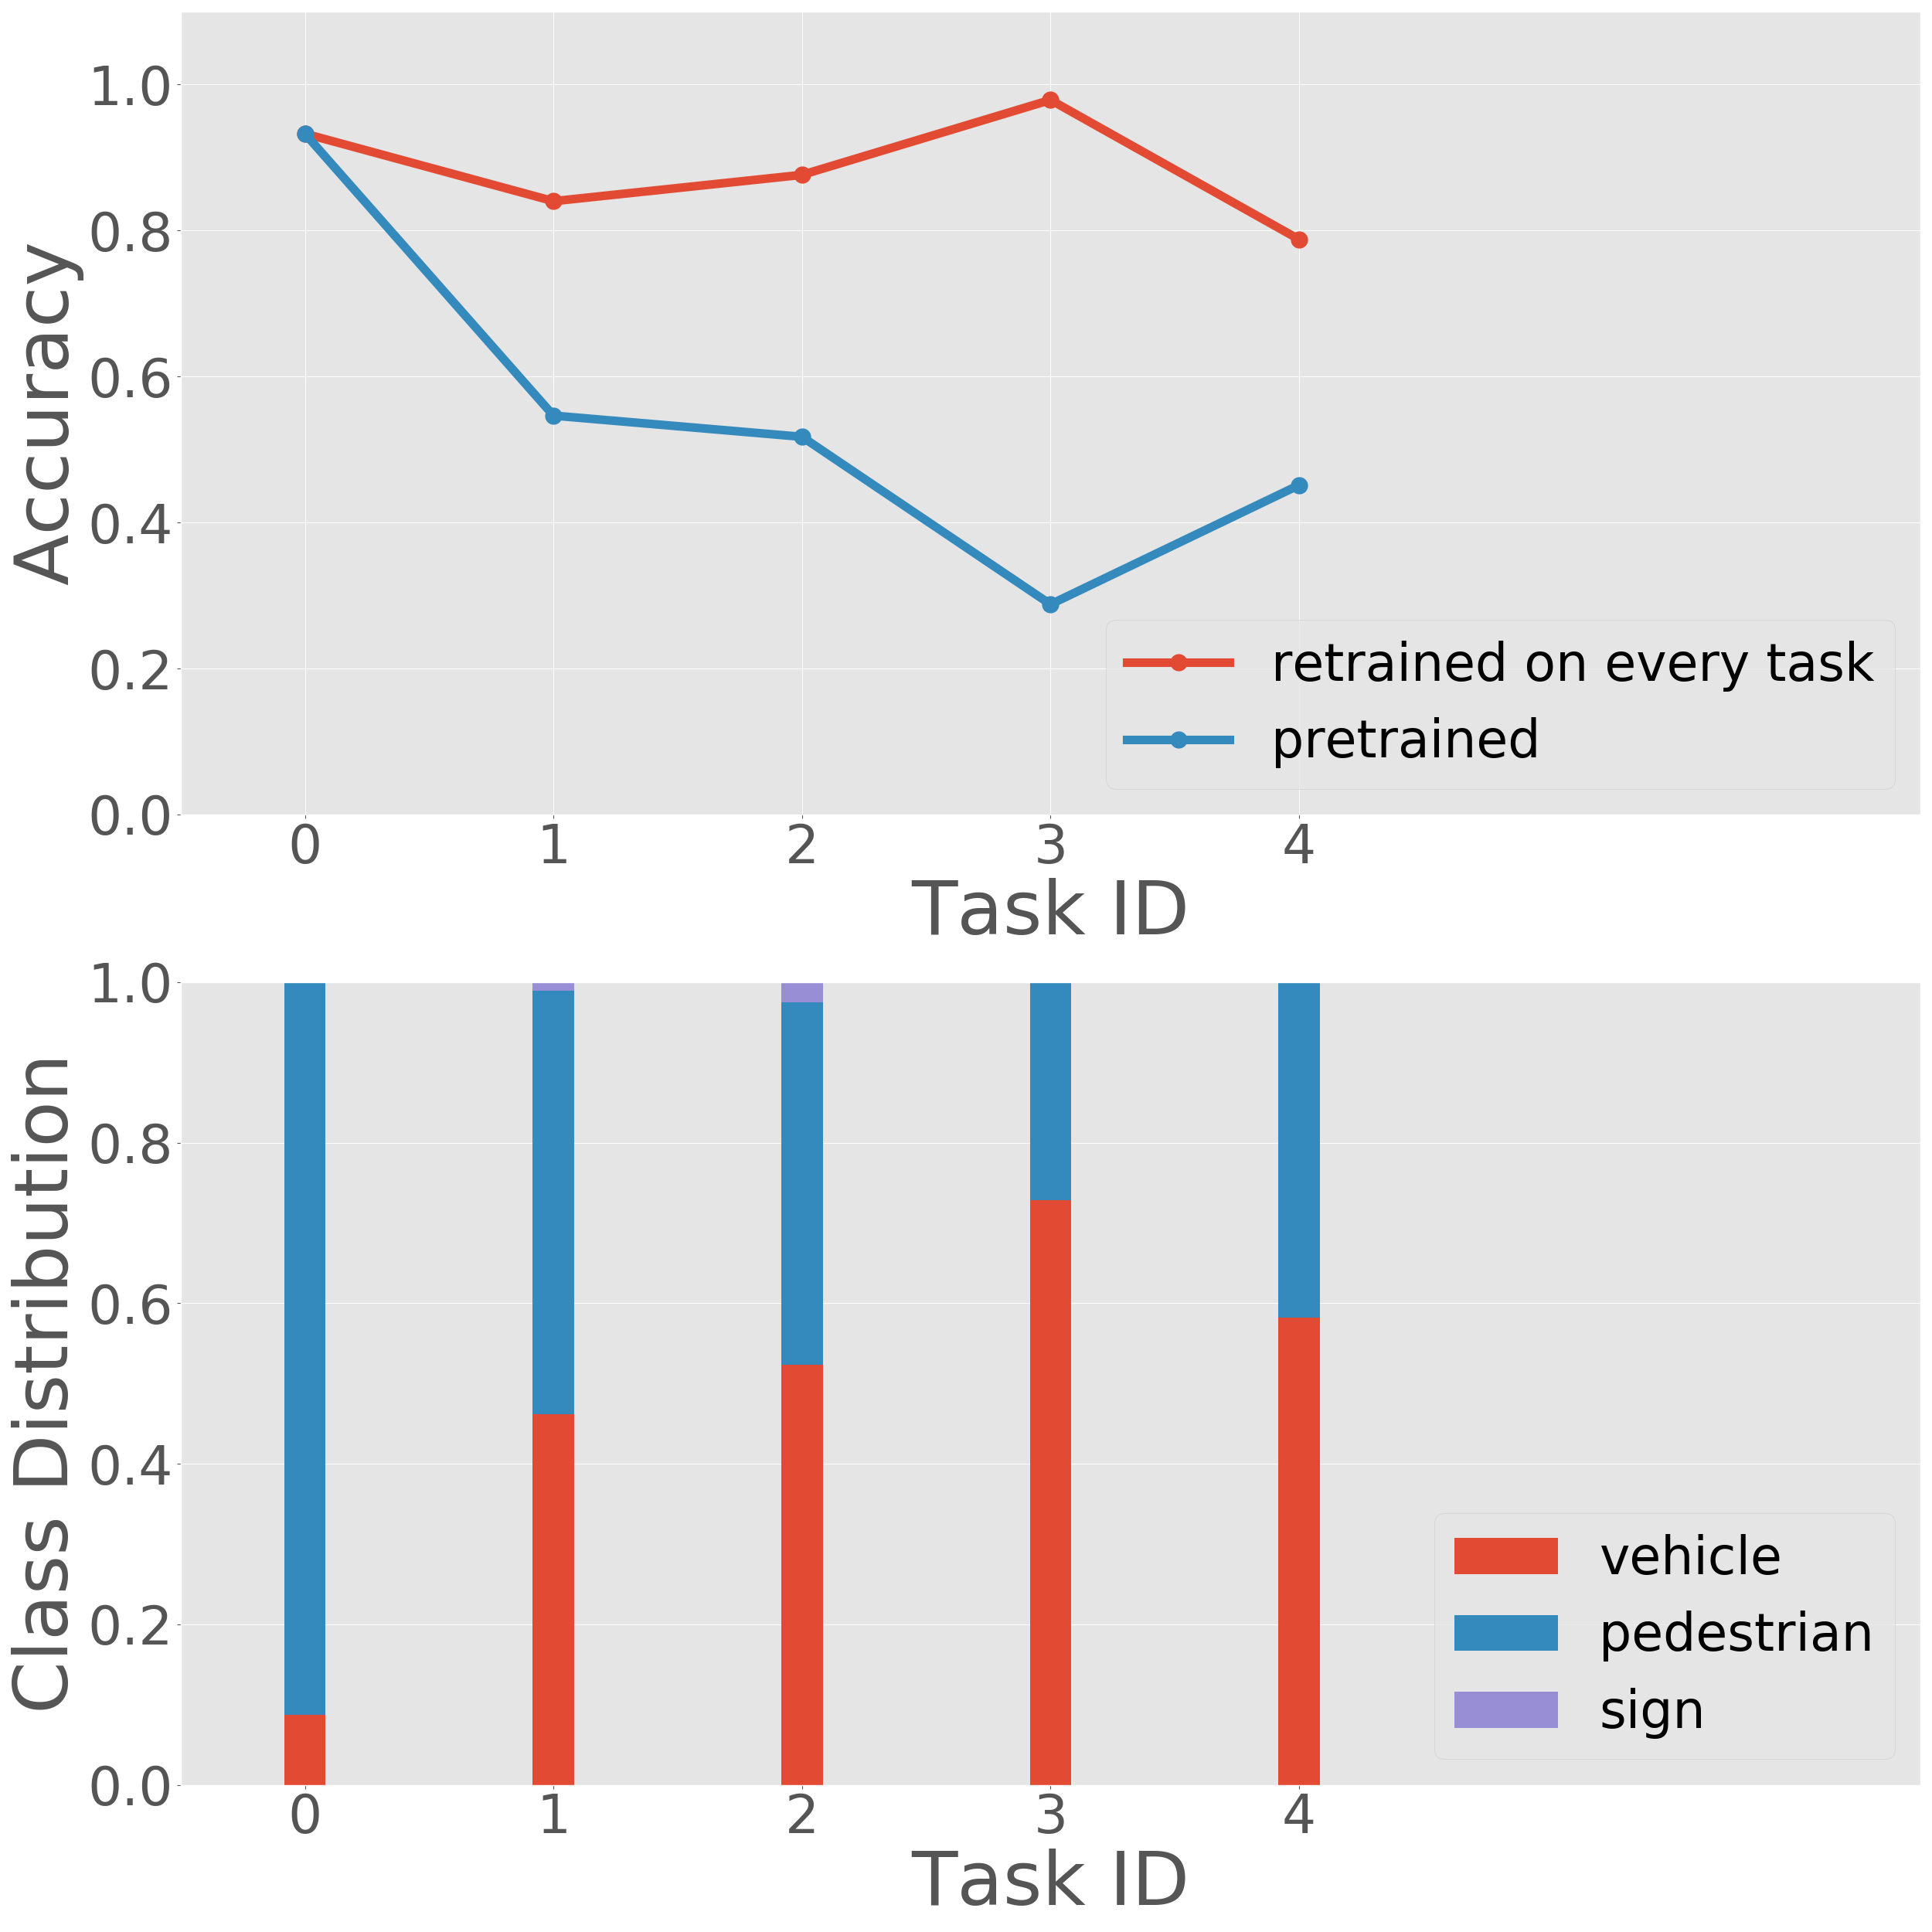
\includegraphics[width=\linewidth]{figures/motivation/Class_Incrementality/class_distribution_change_sf_27.png}
%     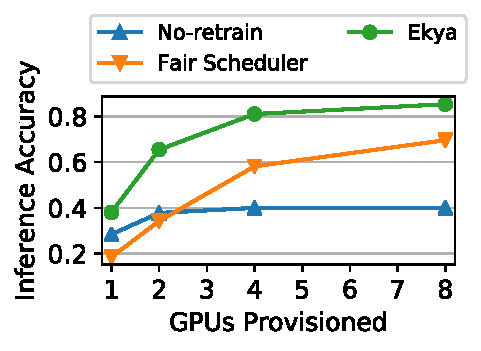
\includegraphics[width=\linewidth]{results/multicam/multicam_acc_vs_res_waymo.pdf}
%      \caption{Waymo}
%     \label{fig:scalability-gpus-waymo}
%   \end{subfigure}
  \begin{subfigure}[t]{0.5\linewidth}
    \centering
    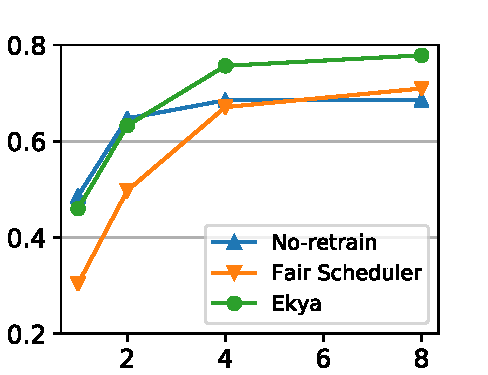
\includegraphics[width=\linewidth]{results/multicam/cityscapes_across_resources.pdf} 
    \caption{Cityscapes}
    \label{fig:scalability-gpus-cityscapes-golden}
  \end{subfigure}
  ~~~
  \begin{subfigure}[t]{0.5\linewidth}
    \centering
    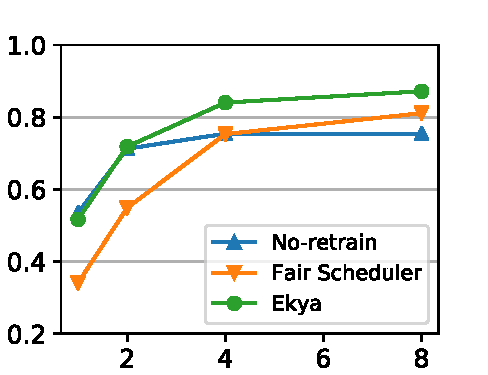
\includegraphics[width=\linewidth]{results/multicam/waymo_across_resources.pdf} 
    \caption{Waymo}
    \label{fig:scalability-gpus-waymo-golden}
  \end{subfigure}
  \caption{\bf Multi-video performance: Our accuracy gain over baselines increases with more GPUs. \romil{Set x,y axis labels and use the custom size params for matplotlib formatting. Reviewer Q.: How do you partition 10 video streams over 8 GPUs?}}
  \label{fig:scalability-gpus}
\end{figure}

\mypara{Accuracy vs. provisioned resource}
Figure~\ref{fig:scalability-gpus} compares the performance of \name, average inference accuracy under same amount of total GPU resource, with the no-retraining baseline and the fair-scheduler baseline.
In each of the Waymo and Cityscapes traces, we randomly pick 10 video streams and run their inference concurrently through five retraining windows.
As we increase the number of provisioned GPUs, we see that \name consistently outperforms the best of the two baselines by a considerable margin
\romilc{xx}\%-\romilc{xx}\% points higher accuracy in Cityscapes and \romilc{xx}\%-\romilc{xx}\% points in Waymo.
Note that these gains in accuracy are achieved without increasing inference delay.
\name allocates resource to retraining only when the accuracy gain from retraining the model outweighs the temporary accuracy drop due to frame subsampling, which explains why \name outperforms the no-retraining baseline. 
Moreover, when \name allocates resource to retraining, it allocates minimum amount needed by the retraining to finish in time, thus outperforming the fair scheduler.
While accuracy gap between \name{} and the fair scheduler baseline decreases as more GPUs are provisioned, \name needs much less resources (upto $6.5\times$ less GPUs, Table \ref{tab::resource-savings-golden}) to achieve the maximum accuracy that fair scheduler attains with 8 GPUs.

%\name's gains over no-retrain baseline are more sizable in Waymo than Cityscapes, but its gains over the fair scheduler baseline are comparable in both traces. 
%This suggests that Waymo data is inherently more suitable for continuous retraining, but through more intelligent resource allocation, \name can always squeeze more juice from retraining than fair scheduler.



% 
\begin{table}[t]
\small
\begin{tabular}{|c|c|c|c|c|}
\hline
\multirow{2}{*}{\begin{tabular}[c]{@{}c@{}}Video\\ Stream\end{tabular}} & \multirow{2}{*}{Accuracy} & \multicolumn{2}{c|}{GPUs Required} & \multirow{2}{*}{\begin{tabular}[c]{@{}c@{}}Resource\\ Savings\end{tabular}} \\ \cline{3-4}
                                                                        &                           & Ekya        & Fair Scheduler       &                                                                             \\ \hline
V0                                                                      & 76.6\%                    & 4           & 13.4                 & $3.3\times$                                                                 \\ \hline
V1                                                                      & 91.5\%                    & 4           & 4.9                  & $1.2\times$                                                                 \\ \hline
V2                                                                      & 78.1\%                    & 4           & 11.2                 & $2.8\times$                                                                 \\ \hline
V3                                                                      & 68.5\%                    & 4           & 14.9                 & $3.7\times$                                                                 \\ \hline
V4                                                                      & 66.9\%                    & 4           & 17.2                 & $4.3\times$                                                                 \\ \hline
V5                                                                      & 81\%                      & 4           & 6.4                  & $1.6\times$                                                                 \\ \hline
V6                                                                      & 80.9\%                    & 4           & 9.4                  & $2.3\times$                                                                 \\ \hline
V7                                                                      & 76.8\%                    & 4           & 15.1                 & $3.7\times$                                                                 \\ \hline
V8                                                                      & 67.8\%                    & 4           & 14.2                 & $3.5\times$                                                                 \\ \hline
V9                                                                      & 67.9\%                    & 4           & 8.9                  & $2.2\times$                                                                \\ \hline
\end{tabular}
\caption{Resource savings for different cities in Cityscapes.}
\label{tab:resource-savings-final}
\end{table}

\begin{table}[t]
\small
\begin{tabular}{|c|c|c|c|c|}
\hline
\multirow{2}{*}{\begin{tabular}[c]{@{}c@{}}Video\\ Stream\end{tabular}} & \multirow{2}{*}{Accuracy} & \multicolumn{2}{c|}{GPUs Required} & \multirow{2}{*}{\begin{tabular}[c]{@{}c@{}}Resource\\ Savings\end{tabular}} \\ \cline{3-4}
                                                                        &                           & Ekya        & Fair Scheduler       &                                                                             \\ \hline
V0                                                                      & 75.6\%                    & 4           & 15.6                 & $3.9\times$                                                                 \\ \hline
V1                                                                      & 78.6\%                    & 4           & 10.0                  & $2.5\times$                                                                 \\ \hline
V2                                                                      & 76.5\%                    & 4           & 19.5                 & $4.9\times$                                                                 \\ \hline
V3                                                                      & 74.5\%                    & 4           & 17.4                 & $4.4\times$                                                                 \\ \hline
V4                                                                      & 75.1\%                    & 4           & 20.9                 & $5.2\times$                                                                 \\ \hline
V5                                                                      & 71.4\%                      & 4           & 25.8                  & $6.5\times$                                                                 \\ \hline
V6                                                                      & 79.5\%                    & 4           & 8.05                  & $2.0\times$                                                                 \\ \hline
V7                                                                      & 75.3\%                    & 4           & 21.8                 & $5.5\times$                                                                 \\ \hline
V8                                                                      & 75.0\%                    & 4           & 84.5                 & $21.1\times$                                                                 \\ \hline
V9                                                                      & 75.2\%                    & 4           & 177.8                  & $44.5\times$                                                                \\ \hline
\end{tabular}
\caption{\bf\small Resource savings for different cities in Cityscapes. \romil{We should write DNF for V7 V8 V9. \romil{This is a bit confusing because every row is not running independently - so this isn't  per resource saving. We should either get overall aggregate number here or run V0 repeatedly to get per video number.}}}
\label{tab:resource-savings-golden}
\end{table}
% gains per stream
\mypara{Performance per video stream}
Figure~\ref{fig:multicam-cities} shows the improvements {\em per video stream} of \name over the baselines, using the same 10 video streams as in Figure~\ref{fig:scalability-gpus} when 4 GPUs provisioned. 
Rather than trading accuracies among video streams, \name re-allocates resources in a way that improves accuracy for {\em all} of the video streams. 
That said, the accuracy gain varies, with gains being more considerable on video streams that have low accuracy without retraining (no-retraining).
This is because these video streams tend to have more dynamic scenes thus may benefit more from retraining.
This highlights a desirable behavior of \name that resource will more likely to be assigned where more accuracy gains are expected.
% \junchen{again, any insight as to what might cause the difference between the two traces?}



% % temporal variance
% \mypara{Timeseries of \name performance}
% Figure~\ref{fig:multicam-timeseries} zooms in on one of the video streams from Figure~\ref{fig:multicam-cities} (V\fillme) and presents the timeseries of performance of \name and the baselines over the five retraining windows. 
% This is one of the video streams that see a high accuracy gain over no-retraining. 
% The timeseries corroborates our intuition: when no-retraining accuracy is low (the \fillme-th retraining window), \name allocates resource to allow it to retrain its model which keeps the accuracy at a high value.

% \begin{figure}
% 	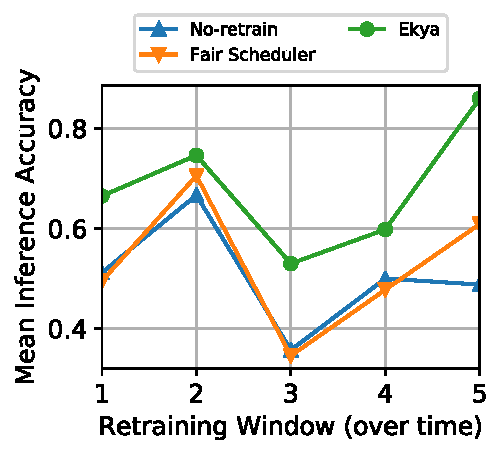
\includegraphics[width=0.4\textwidth]{results/multicam/multicam_taskwise_acc_zurich_4_cityscapes.pdf}
% 	\caption{\bf Timeseries of our performance vs. fair sharing. Again, adaptive resource sharing constantly outperforms fair sharing. \romil{Accuracy drops over time.}}
% 	\label{fig:multicam-timeseries}
% \end{figure}


% scalability: with more gpus, we can support more camera
\mypara{Scalability with more GPUs}
Next, we evaluate the scalability of \name's {\em throughput} as more GPUs are available.
We define throughput as the maximum number of video streams that can run concurrently on the GPUs while achieving a accuracy within a threshold of the maximum possible mean accuracy.
(This definition is common in practice, since applications usually require accuracy to be above a threshold for the inference to be usable.)
Figure~\ref{fig:scalability-gpu-vs-cam-thresholded} shows that \name's throughput grows almost linearly with more available GPUs, and at a rate \romilc{$2.3\times$} faster than the baseline of fair scheduler.
This suggests that \name can more easily scale to a large number of video sources than the baselines.

\begin{figure}
  \centering
%   \begin{subfigure}[t]{\linewidth}
%     \centering
%     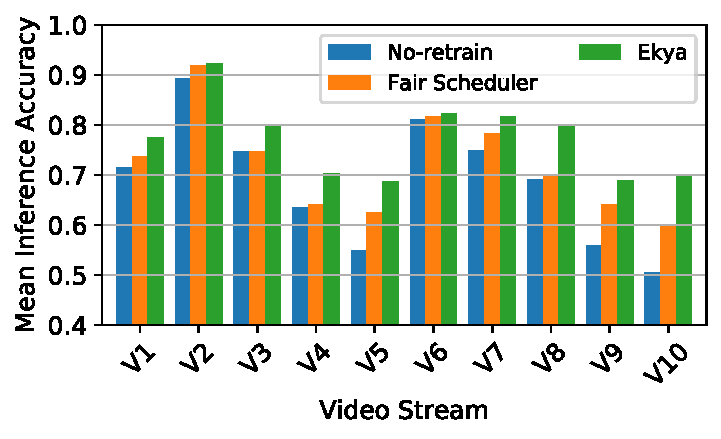
\includegraphics[width=0.9\linewidth]{results/multicam/multicam_individual_stream_acc_cityscapes.pdf} 
%     \caption{Cityscapes Human Label}
%     %\label{fig:multicam-cities-cityscapes}
%   \end{subfigure}
    \begin{subfigure}[t]{\linewidth}
    \centering
    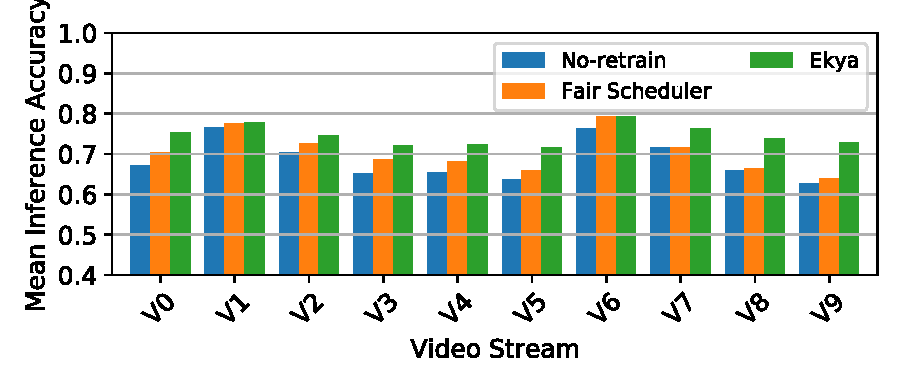
\includegraphics[width=0.9\linewidth]{results/multicam/cityscapes_across_cities.pdf} 
    %\caption{Cityscapes Golden Model}
    %\label{fig:multicam-cities-cityscapes}
  \end{subfigure}
%   ~~~
%   \begin{subfigure}[t]{0.5\linewidth}
%     \centering
%     % 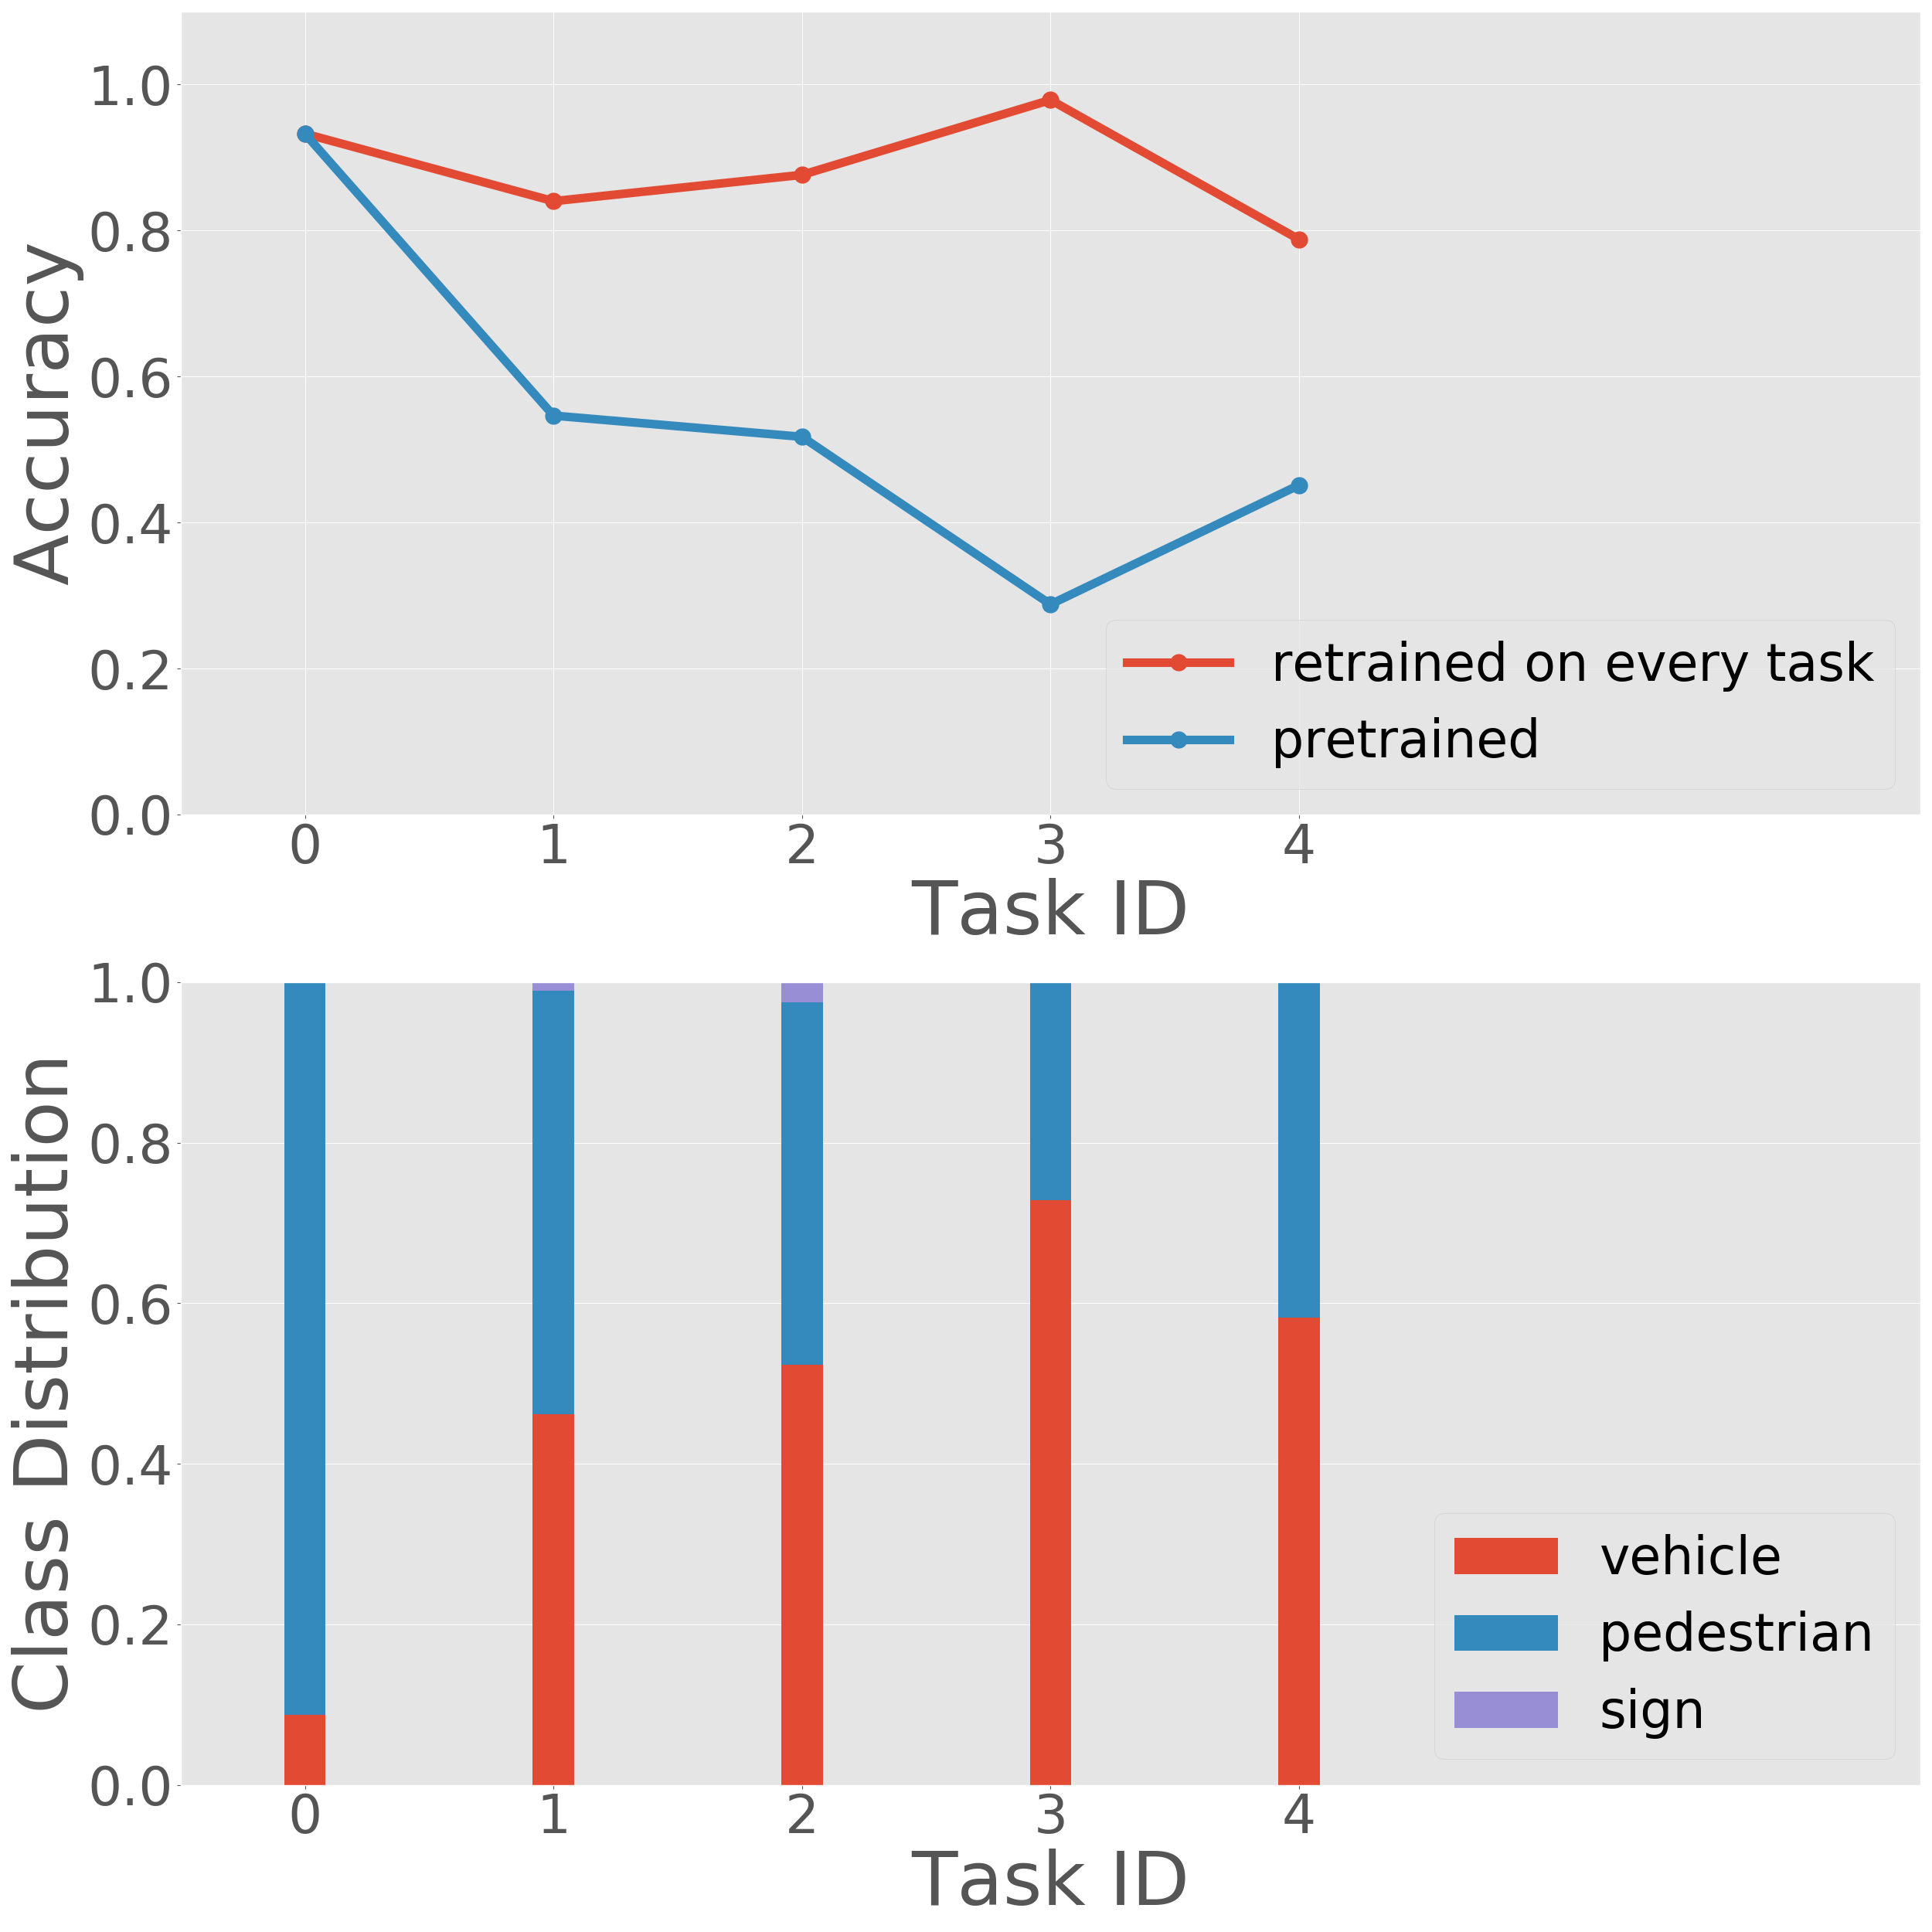
\includegraphics[width=\linewidth]{figures/motivation/Class_Incrementality/class_distribution_change_sf_27.png}
%     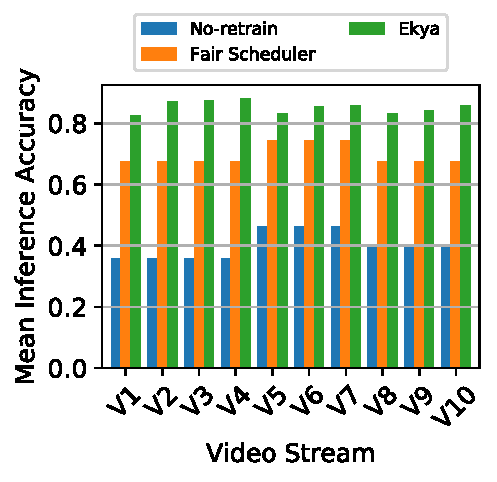
\includegraphics[width=\linewidth]{results/multicam/multicam_individual_stream_acc_waymo.pdf}
%      \caption{Waymo}
%     \label{fig:multicam-cities-waymo}
%   \end{subfigure}
  \caption{Multi-video performance: Ours (with continuous retraining) vs. Fair Share Scheduler. Compared across cities, we do consistently better. Some cities see bigger gains than others, which are thus prioritized by \name{}.}
  \label{fig:multicam-cities}
\end{figure}


Figure \ref{fig:scalability-fixedGPUs-accuracy} evaluates the throughput-accuracy tradeoff made by \name{} with a fixed number of resources. To minimize the accuracy variations between cities, we add video streams by replicating a fixed video stream from the Cityscapes dataset. 
With only a single GPU, increasing the number of video streams forces \name{} to gradually reduce resource allocation to retraining in favour of keeping of a high inference accuracy by allocating all resources to inference. The fair scheduler is unaware of the resource cost of retraining, and diverts GPU cycles from inference, resulting a lower inference accuracy.

\begin{figure}
 	%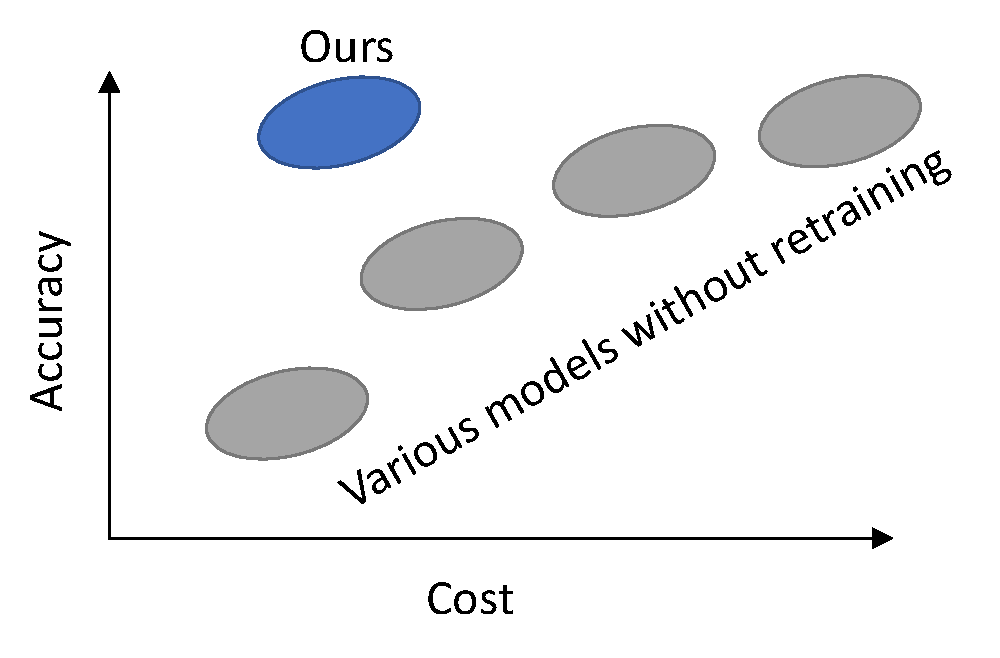
\includegraphics[width=0.4\textwidth]{figures/eval_placeholders/single-tradeoffs.pdf}
 	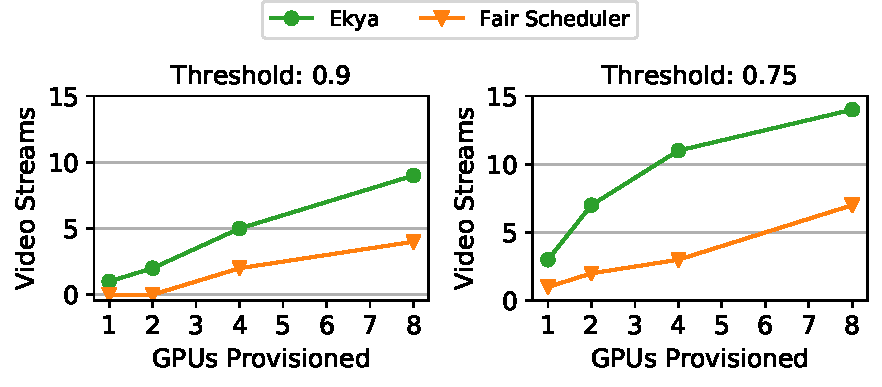
\includegraphics[width=\linewidth]{results/scalability/scalability_GPUs_cams_cityscapes.pdf}
	\caption{\bf Throughput measured as number of video streams that can be concurrently supported for different resource sizes subject to accuracy thresholds.
	%The accuracy threshold is a multiplicative factor of the maximum achievable mean accuracy for a workload given $\infty$ resources.
	}
	\label{fig:scalability-gpu-vs-cam-thresholded}
\end{figure}

% SIGCOMM Results:
% \begin{figure}
%  	%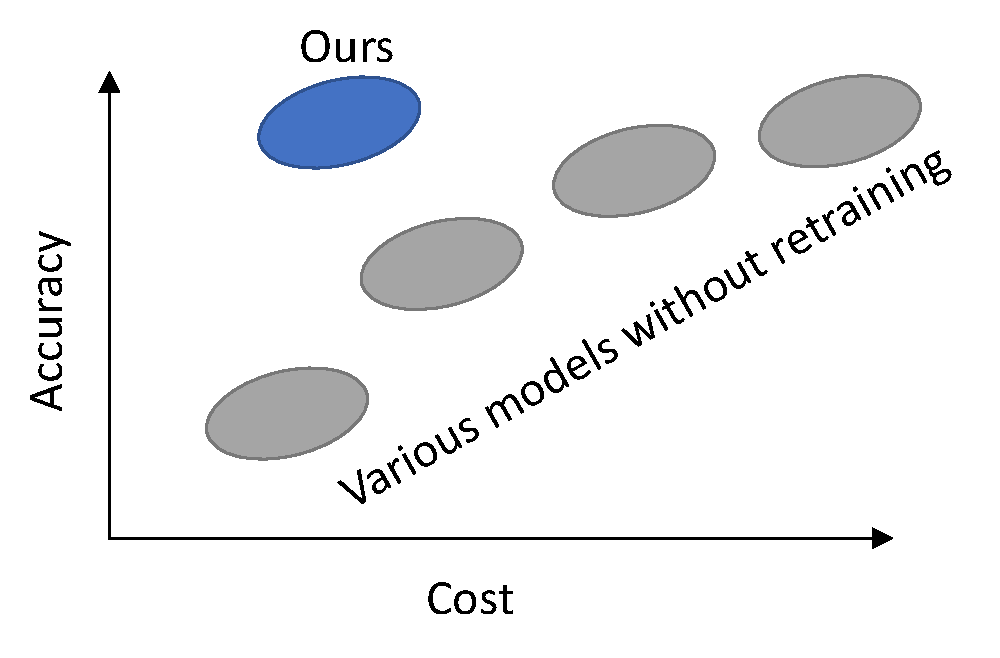
\includegraphics[width=0.4\textwidth]{figures/eval_placeholders/single-tradeoffs.pdf}
%  	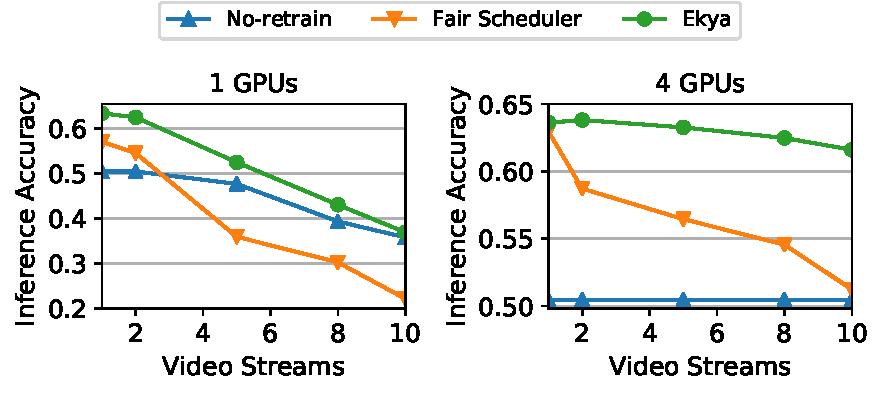
\includegraphics[width=\linewidth]{results/scalability/scalability_cams_fixedGPUs_cityscapes.pdf}
% 	\caption{\bf Effect of adding more video streams on accuracy for different schedulers. When insufficient resources are provisioned, \name{} gracefully degrades to the No-retrain baseline, while the retraining decisions made by the fair scheduler reduce the mean inference accuracy.}
% 	\label{fig:scalability-fixedGPUs-accuracy}
% \end{figure}
\begin{figure}
 	%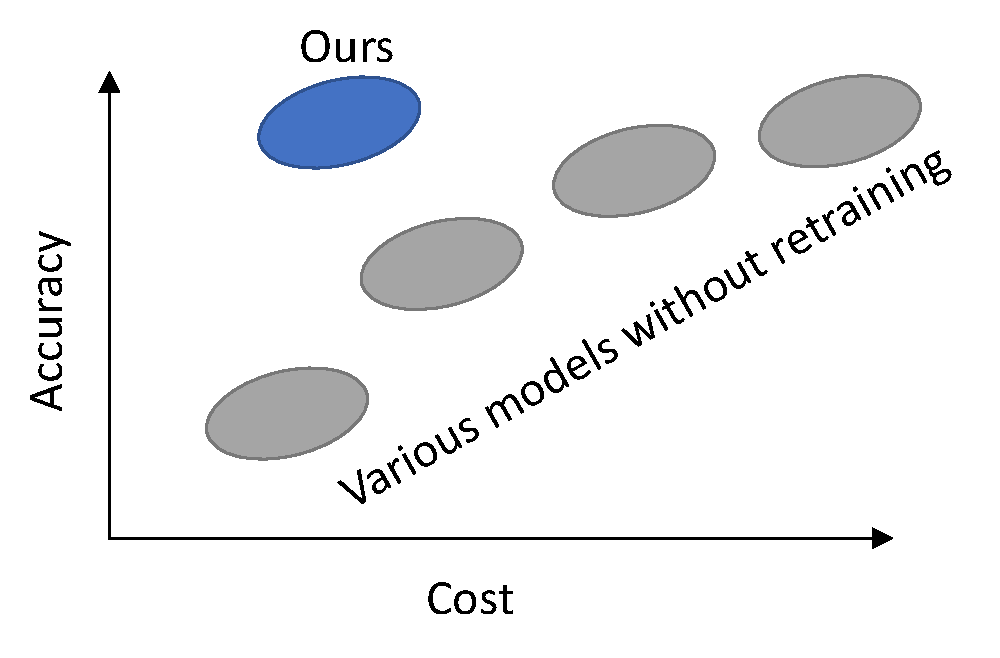
\includegraphics[width=0.4\textwidth]{figures/eval_placeholders/single-tradeoffs.pdf}
 	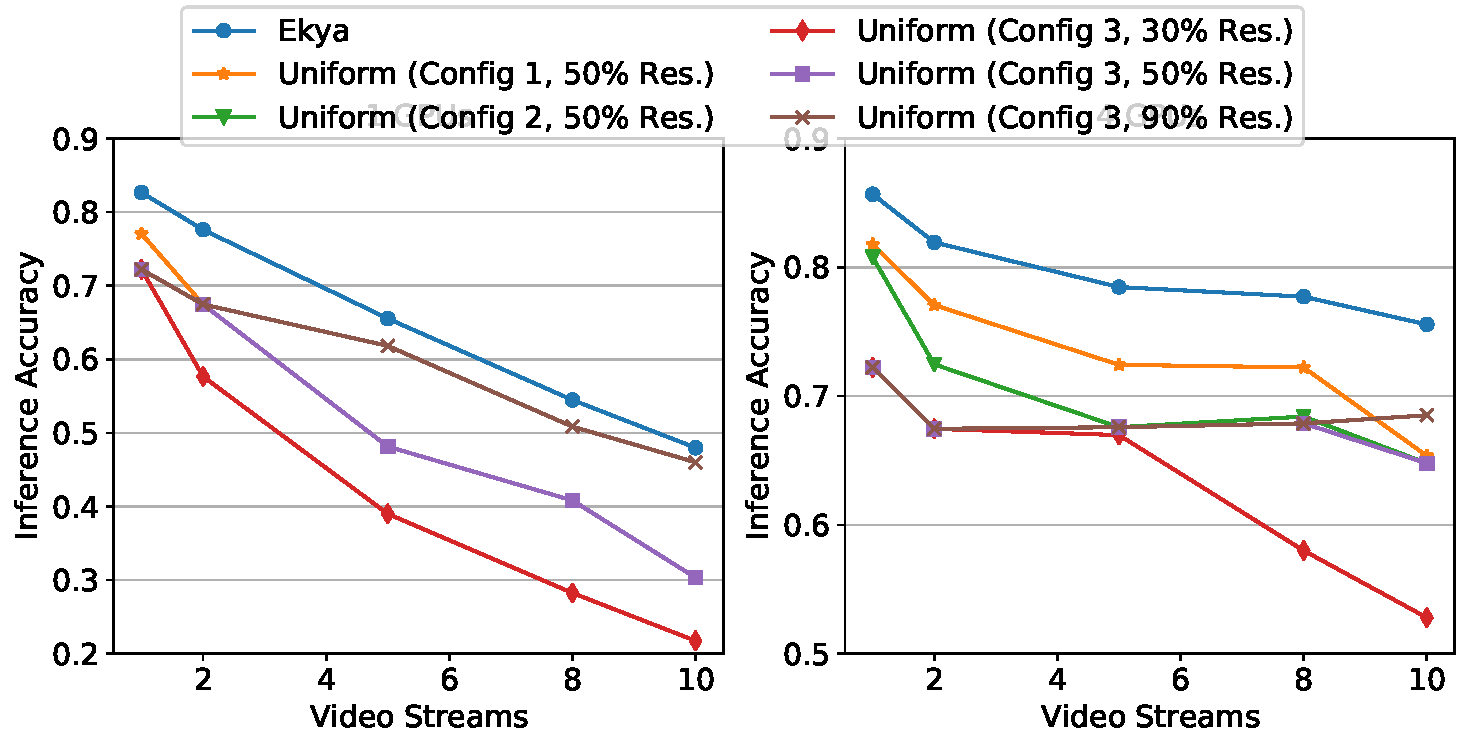
\includegraphics[width=\linewidth]{results/scalability/scalability_cams_fixedGPUs_cityscapes_golden_model.pdf}
	\caption{\bf Using golden model. Effect of adding more video streams on accuracy for different schedulers. When insufficient resources are provisioned, \name{} gracefully degrades to the No-retrain baseline, while the retraining decisions made by the fair scheduler reduce the mean inference accuracy.}
	\label{fig:scalability-fixedGPUs-accuracy}
\end{figure}


% per video. even if one video, gains are impressive
\mypara{Gains with single video stream}
Figure~\ref{fig:singlecam-cities} presents the same analysis of Figure~\ref{fig:scalability-gpus} but with only one video stream using the resources.
Across these video streams (and many others but not shown), we see that \name consistently outperforms the baselines by dynamically deciding when to retrain the model as well as the resource balance between retraining and inference.
As in Figure~\ref{fig:multicam-cities}, we see the gains vary considerably across video streams, which again highlights that some video streams can inherently benefit more from retraining.% their models.

% \begin{figure}
%   \centering
%   \begin{subfigure}[t]{\linewidth}
%     \centering
%     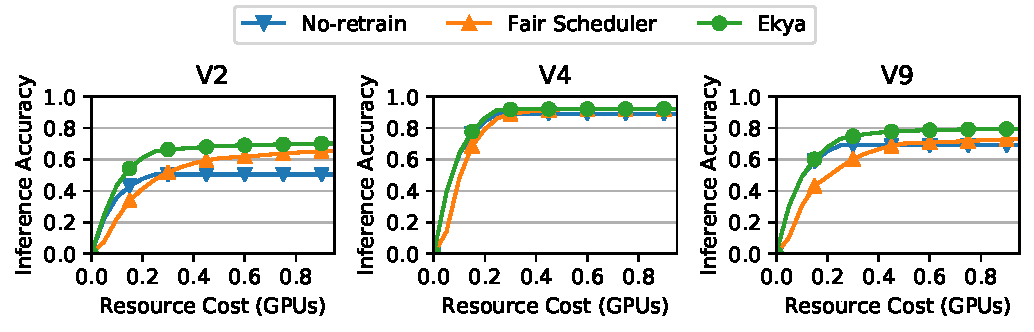
\includegraphics[width=\linewidth]{results/singlecam/singlecam_acc_vs_cost_cityscapes.pdf} 
%     \caption{Cityscapes}
%     \label{fig:singlecam-cities-cityscapes}
%   \end{subfigure}
%   \hfill
%   \begin{subfigure}[t]{\linewidth}
%     \centering
%     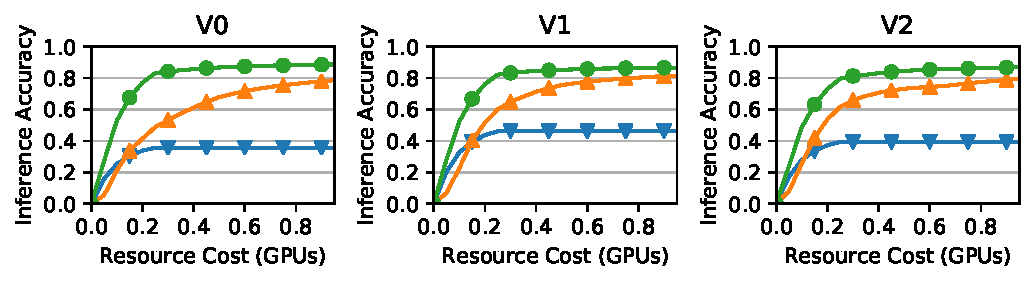
\includegraphics[width=\linewidth]{results/singlecam/singlecam_acc_vs_cost_waymo.pdf}
%     \caption{Waymo}
%     \label{fig:singlecam-cities-waymo}
%   \end{subfigure}
%   \caption{Single-video performance - different videos have different payoffs for retraining.}% In \ref{fig:singlecam-cities-cityscapes}, V2 demonstrates large benefits to retraining compared to V4.}
%   \label{fig:singlecam-cities}
% \end{figure}

\begin{figure}
  \centering
  \begin{subfigure}[t]{\linewidth}
    \centering
    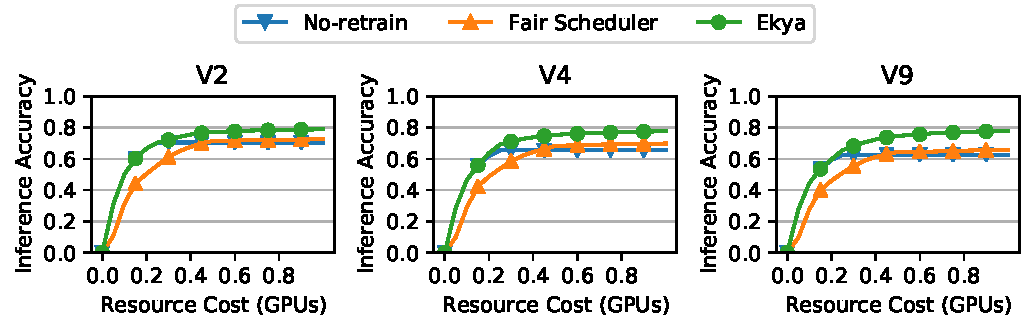
\includegraphics[width=\linewidth]{results/singlecam/singlecam_acc_vs_cost_golden_cityscapes.pdf} 
    \caption{Cityscapes}
    \label{fig:singlecam-cities-cityscapes-golden}
  \end{subfigure}
  \hfill
  \begin{subfigure}[t]{\linewidth}
    \centering
    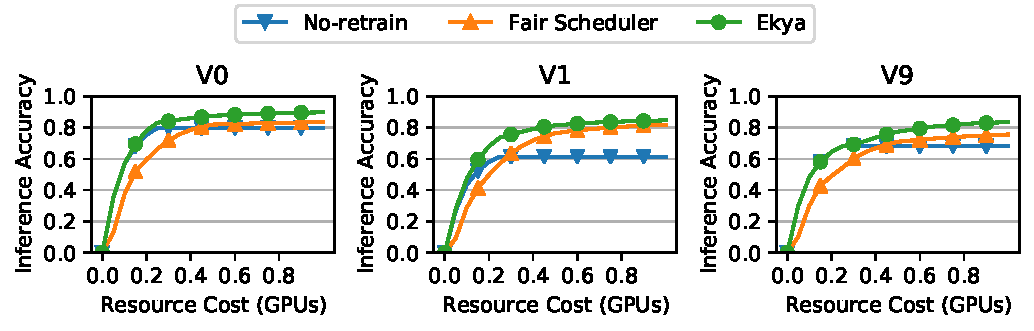
\includegraphics[width=\linewidth]{results/singlecam/singlecam_acc_vs_cost_golden_waymo.pdf}
    \caption{Waymo}
    \label{fig:singlecam-cities-waymo-golden}
  \end{subfigure}
  \caption{Single-video performance - different videos have different payoffs for retraining.}% In \ref{fig:singlecam-cities-cityscapes}, V2 demonstrates large benefits to retraining compared to V4.}
  \label{fig:singlecam-cities}
\end{figure}


\subsection{Comparison with alternative designs}
\label{subsec:eval-alternate}

Next, we evaluate two alternative designs for continuous retraining---(1) re-using a retrained model from a history window that shares class distribution (instead of retraining the model again) and (2) offloading the retraining to the cloud.

\mypara{Advantage over re-using cached models}
Reusing a cached model from history is tempting as it avoids the cost of model retraining. 
%Figure~\ref{fig:history-vs-current} compares 
We compare the accuracy of retraining the model on the current window (\name) with the accuracy of re-using the model from a history window in which the class distribution is close to the distribution in the current window (Euclidean distance $\leq 0.2$; \S\ref{sec:profiling}). Here we use ResNet18 as the model and Waymo as the trace.
%The graph, however, shows 
We observe that 
the accuracy is much lower by re-using the model from history, even when the history window share a similar class distribution. At median, the difference in accuracy is 11\% with the $90^\text{th}$ percentile and maximum divergence in accuracies being as high as $38\%$ and $51\%$. 
This confirms our intuition in \S\ref{sec:profiling} that although sharing a similar class distribution is indicative of the difficulty of retraining, it does not mean the model can be directly reused from any window with similar class distribution.


%\begin{figure}[t!]
%\centering
%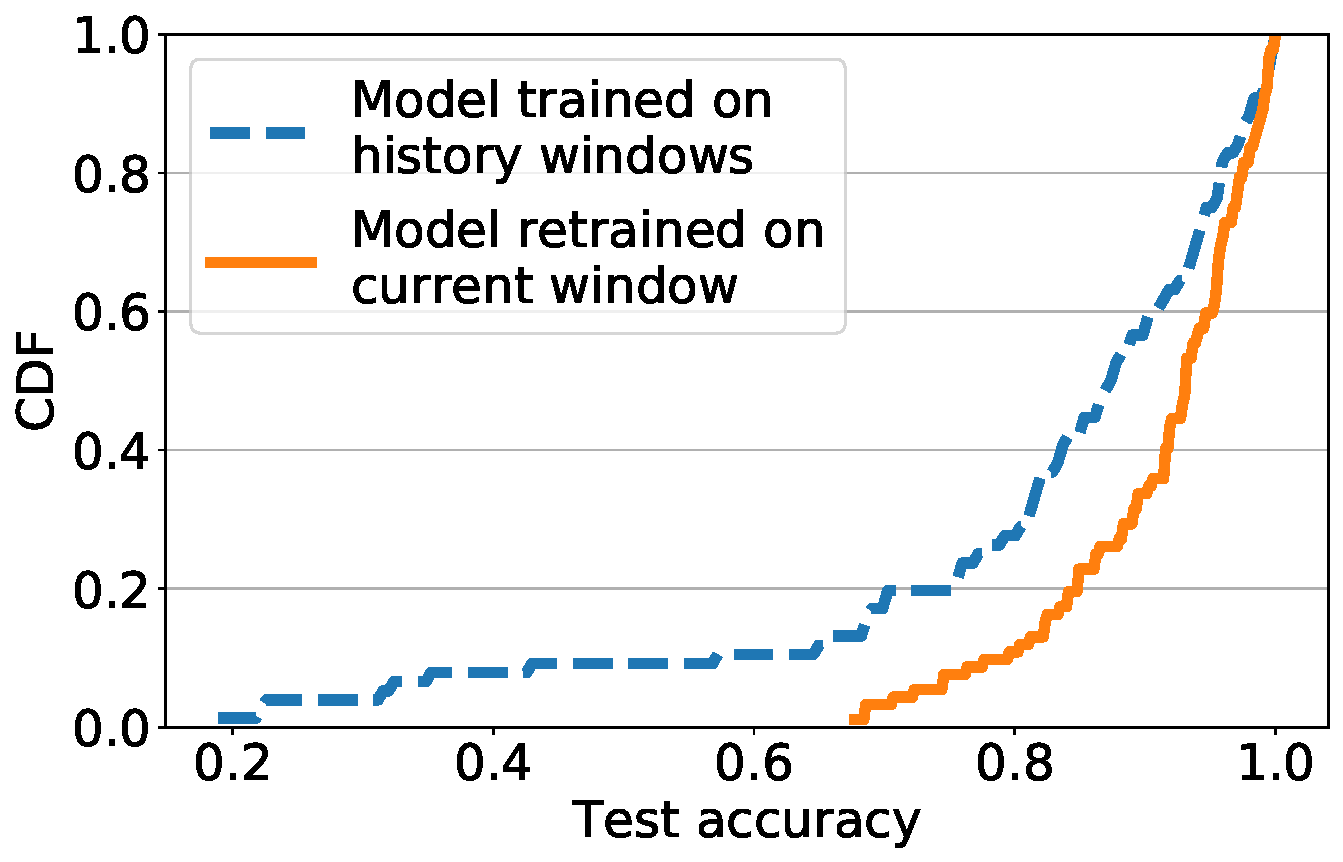
\includegraphics[width=0.6\columnwidth]{figures/eval_placeholders/history-trained-vs-retrained-cdf.pdf}
%\vspace{-0.2cm}
%\caption{Gap between accuracy of the model retrained in the current and accuracy of re-using a model retrained in a history window that share similar class distribution.
%\vspace{-0.2cm}}
%\label{fig:history-vs-current}
%\end{figure}


\mypara{Advantage over a cloud-based solution}
Retraining could be offloaded to the cloud so the edge servers can focus on inference, but on a closer look such a cloud-based solution will even negate the benefit of retraining the model, because of the expensive communication delay from uploading training data to the cloud and downloading retrained models). 

%It is fundamentally challenging to run continuous learning across the edge-cloud because of network constraints.

% Math sheet new - https://docs.google.com/spreadsheets/d/1-WDeFmQwHy0sEpxL9f6QcbMKt1DVPaX6ODjMwDbb3IY/edit#gid=0
For instance, consider a setup serving 5 video streams in parallel with a retraining window size of 400 seconds. For a bit rate of 8 Mbps \cite{bitrate} and assuming a 10\% subsampling, it amounts to 320 Mb of training data being generated per camera in every retraining window. This retraining data must be uploaded to cloud and a model must be retrained and fetched back to the edge. Uploading 320 Mb over an average cellular uplink of 5.1 Mbps \cite{opensignal_2018} for 5 cameras results in a total upload time of 313 seconds. A model checkpoint of ResNet18 is 398 Mb, downloading which would take 23 seconds per camera on a downlink of 17.3 Mbps \cite{opensignal_2018}, or a total of 115 seconds for 5 cameras. The total network transfer cost is 428 seconds, which exceeds the retraining window size of 400 seconds. 

% Mention do we have to send everything to the cloud.

% examples where the drop is higher
Even on provisioning double the bandwidth (which entails an expensive change of the network link from cellular to cable), retraining on the cloud does not yield a higher accuracy in our simulator. We extend our simulator to simulate the network delays and assume that the the cloud offers a speed up of $10\times$ and has infinite parallel resources. Even then, the cloud \romilc{RTT} takes about 216 seconds and yields a mean inference accuracy of 81.8\%. In contrast, retraining at the edge completes in 125 seconds, leaving more time to take advantage of the retraining model, and results in an inference accuracy of 83.75\%.

% Show the calculation
% Mention the cost
% Varying network connections
Achieving the same accuracy in our simulations required increasing the downlink and uplink bandwidth by $3\times$ and still operates under the assumption that the cloud can provision parallel resources instantly, which can be expensive.

% Math sheet- https://docs.google.com/spreadsheets/d/1z4Zui8Qmg4iH-_yQKu7p0EZtXOlj_-ogKIW9mbf-Tpo/edit#gid=179811194

% For instance, each retraining window in the Waymo dataset accumulates about 1760 Mb of data every 20 seconds, resulting in a 88 Mb/s bitrate. Assuming a 10\% sub-sampling rate for retraining and a retraining window of 200 seconds (as in all our experiments), a total of 1760 Mb  of training data must be sent to the cloud. With an uplink of 5.1 Mb/s \cite{opensignal_2018}, just uploading the training data would take 345 seconds. Moreover, the updated model weights need to be downloaded from the cloud, which is 360 Mb in size. With a downlink throughput of 17.3 Mb/s \cite{opensignal_2018} (cellular connection), that adds another 20 seconds. Combined, this results in nearly 365s to get the retrained model, which far exceeds the retraining window size of 5 minutes (note that we have ignored the time to run the training in the cloud). Since even the sub-sampled video bitrate exceeds the limited bandwidths at the edge, this analysis applies for all retraining window sizes.


% \junchen{i still feel this should be in motivation section, no?}

\subsection{Sensitivity analysis}
\label{subsec:sensitivity-eval}

% \begin{figure} [t!]
%  	%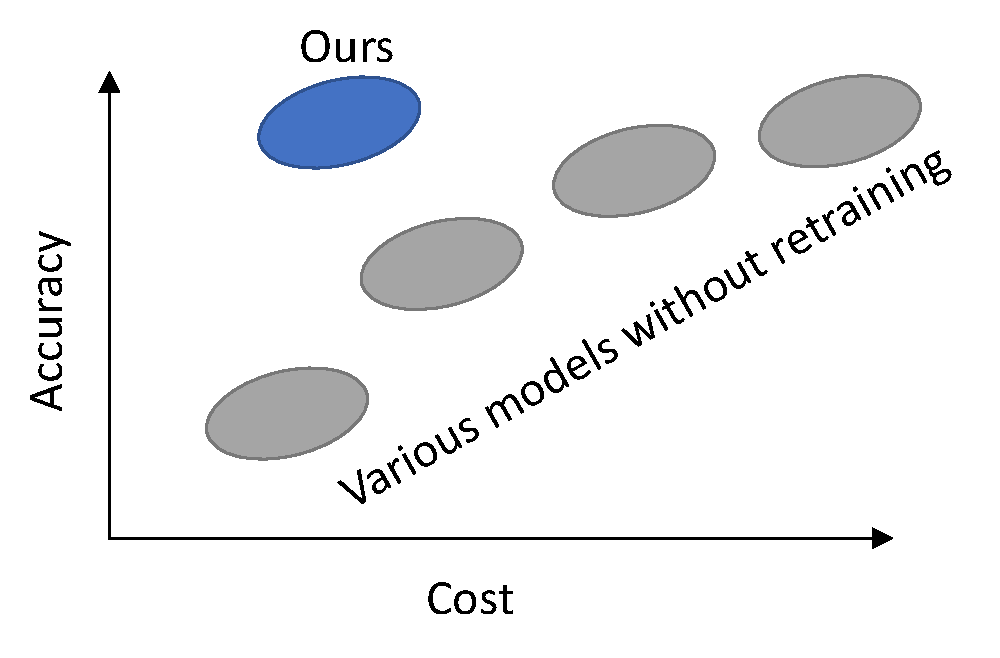
\includegraphics[width=0.4\textwidth]{figures/eval_placeholders/single-tradeoffs.pdf}
%  	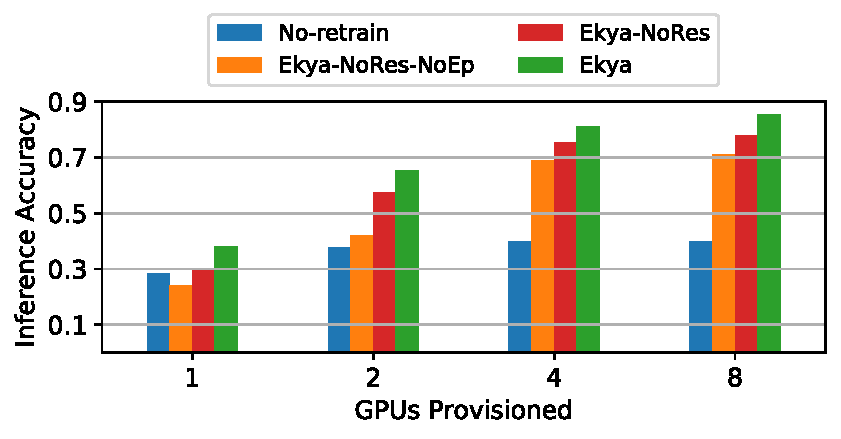
\includegraphics[width=\linewidth]{results/ablation_waymo.pdf}
% 	\caption{\bf {\name} factor analysis by removing  dynamic resource allocation and reducing the hyperparameter space.}
% 	\label{fig:factor-analysis}
% \end{figure}

\begin{figure} [t!]
 	%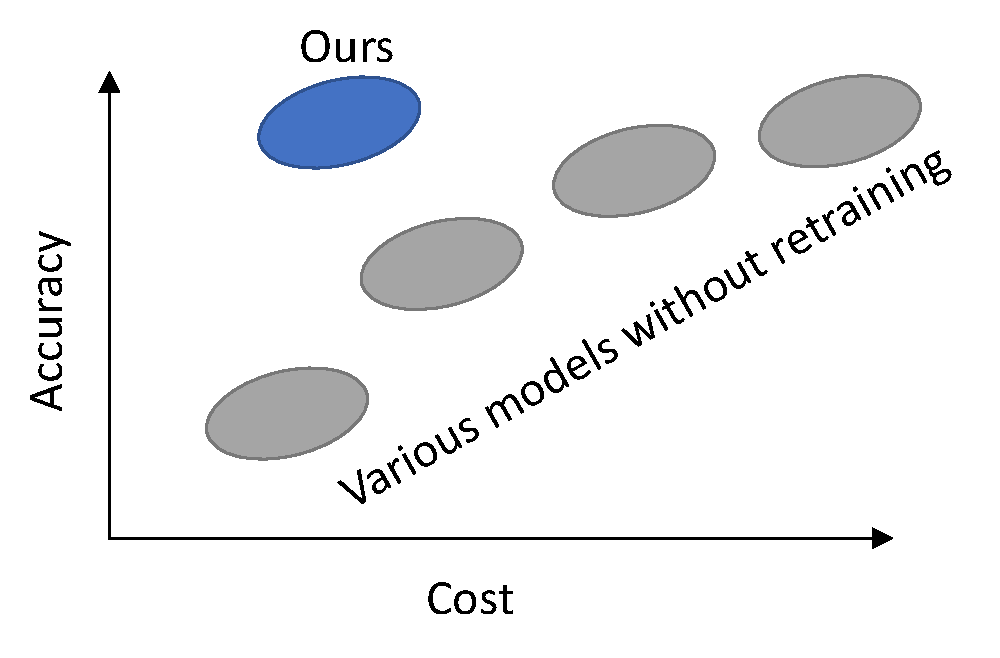
\includegraphics[width=0.4\textwidth]{figures/eval_placeholders/single-tradeoffs.pdf}
 	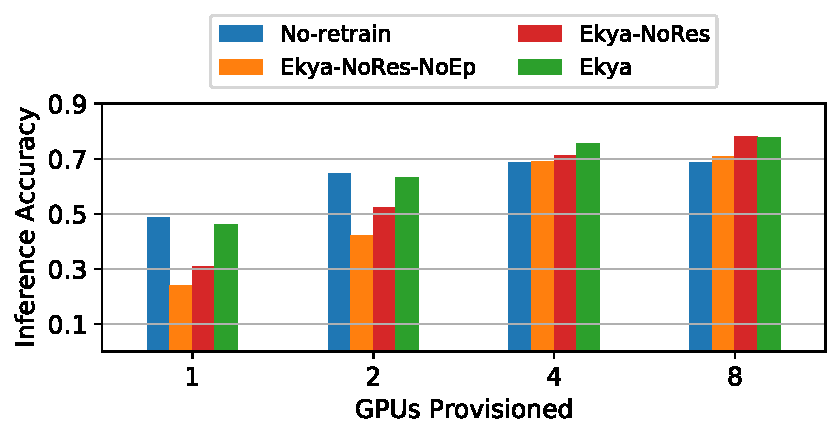
\includegraphics[width=\linewidth]{results/ablation_cityscapes_golden.pdf}
	\caption{\bf {\name} factor analysis by removing  dynamic resource allocation and reducing the hyperparameter space.}
	\label{fig:factor-analysis}
\end{figure}

% improvement breakdown
\mypara{Factor analysis}
To understand the contribution of each part of \name, we run a factor analysis on the same setting as Figure~\ref{fig:scalability-gpus} (10 video streams with 4 GPUs provisioned). We construct two schedulers from {\name}. \emph{Ekya-NoRes}, which removes the smart resource allocation in \name. \emph{Ekya-NoRes-NoEp} removes resource allocation and additionally fixes the number of epochs a model is trained to the maximum value, effectively removing it from the configuration space. We chose this hyperparameter for removal because it creates the largest diversity in the resource-accuracy profiles of configurations. 

As observed in Figure \ref{fig:factor-analysis}, the diversity in configurations and their careful selection has a large contribution to \name{}'s gains in accuracy when fewer resources are provisioned, which reduces as more resources are made available. This is because with more resources, even expensive configurations become feasible, thus configuration selection matters less. The smart resource allocation mechanism in {\name} has a nearly consistent contribution to \name{}'s performance.

%We note that the accuracy of \emph{Ekya-NoRes-NoEp} is lower than \emph{No-retrain} when 1 GPU is provisioned because resource reallocation is removed, and thus it always allocates resources to retraining. It just so happens that there are no good configurations to pick from once the epochs hyperparameter is removed, and thus the accuracy is lesser than \emph{No-retrain}.



% sensivity to accuracy errors
\mypara{Sensitivity to accuracy estimation errors}
\romil{Add paragraph and plot on accuracy of microprofiling.} %Resource consumption and accuracy of accuracy estimation. E
We now test the impact of errors in accuracy profiles (\S\ref{subsec:profiling}) on \name's performance gains.
To control the amount of errors, we add a controlled Gaussian noise on top of the real retraining accuracy as the predictions when the profiler is queried. 
Figure~\ref{fig:sensitivity-accuracy-error} shows that with upto 20\% errors in the profiler prediction, the maximum accuracy drop is 3\% points. When a 50\% profiling error is introduced, the accuracy drop is 7.9\% points. Such a large profiling error makes \name{} worse than the no-retrain baseline, but still better than fair scheduling.

\begin{figure}
	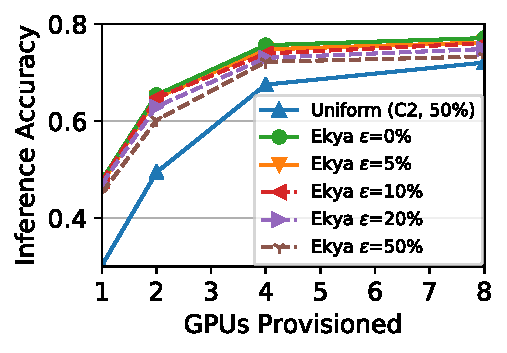
\includegraphics[width=\linewidth]{results/sensitivity/sensitivity_profileerrors_cityscapes.pdf}
	\caption{\bf Adding a controlled error $\epsilon$ to the accuracy prediction -  \name{}'s performance degrades, but only marginally.}
	\label{fig:sensitivity-accuracy-error}
\end{figure}

% Two subfigure plot for sensitivity 
% \begin{figure}
%   \centering
%   \begin{subfigure}[t]{0.5\linewidth}
%     \centering
%     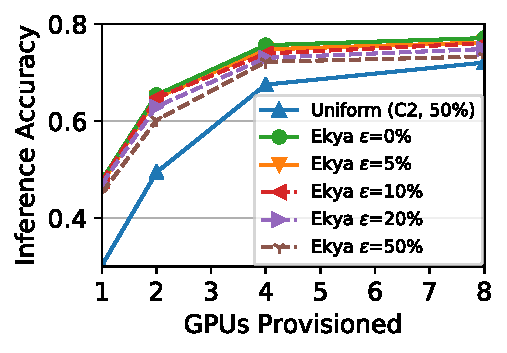
\includegraphics[width=\linewidth]{results/sensitivity/sensitivity_profileerrors_cityscapes.pdf} 
% 	\caption{\bf Adding errors to the profiler.}
%     \label{fig:sensitivity-accuracy-error}
%   \end{subfigure}
%   ~~~
%   \begin{subfigure}[t]{0.5\linewidth}
%     \centering
%     % 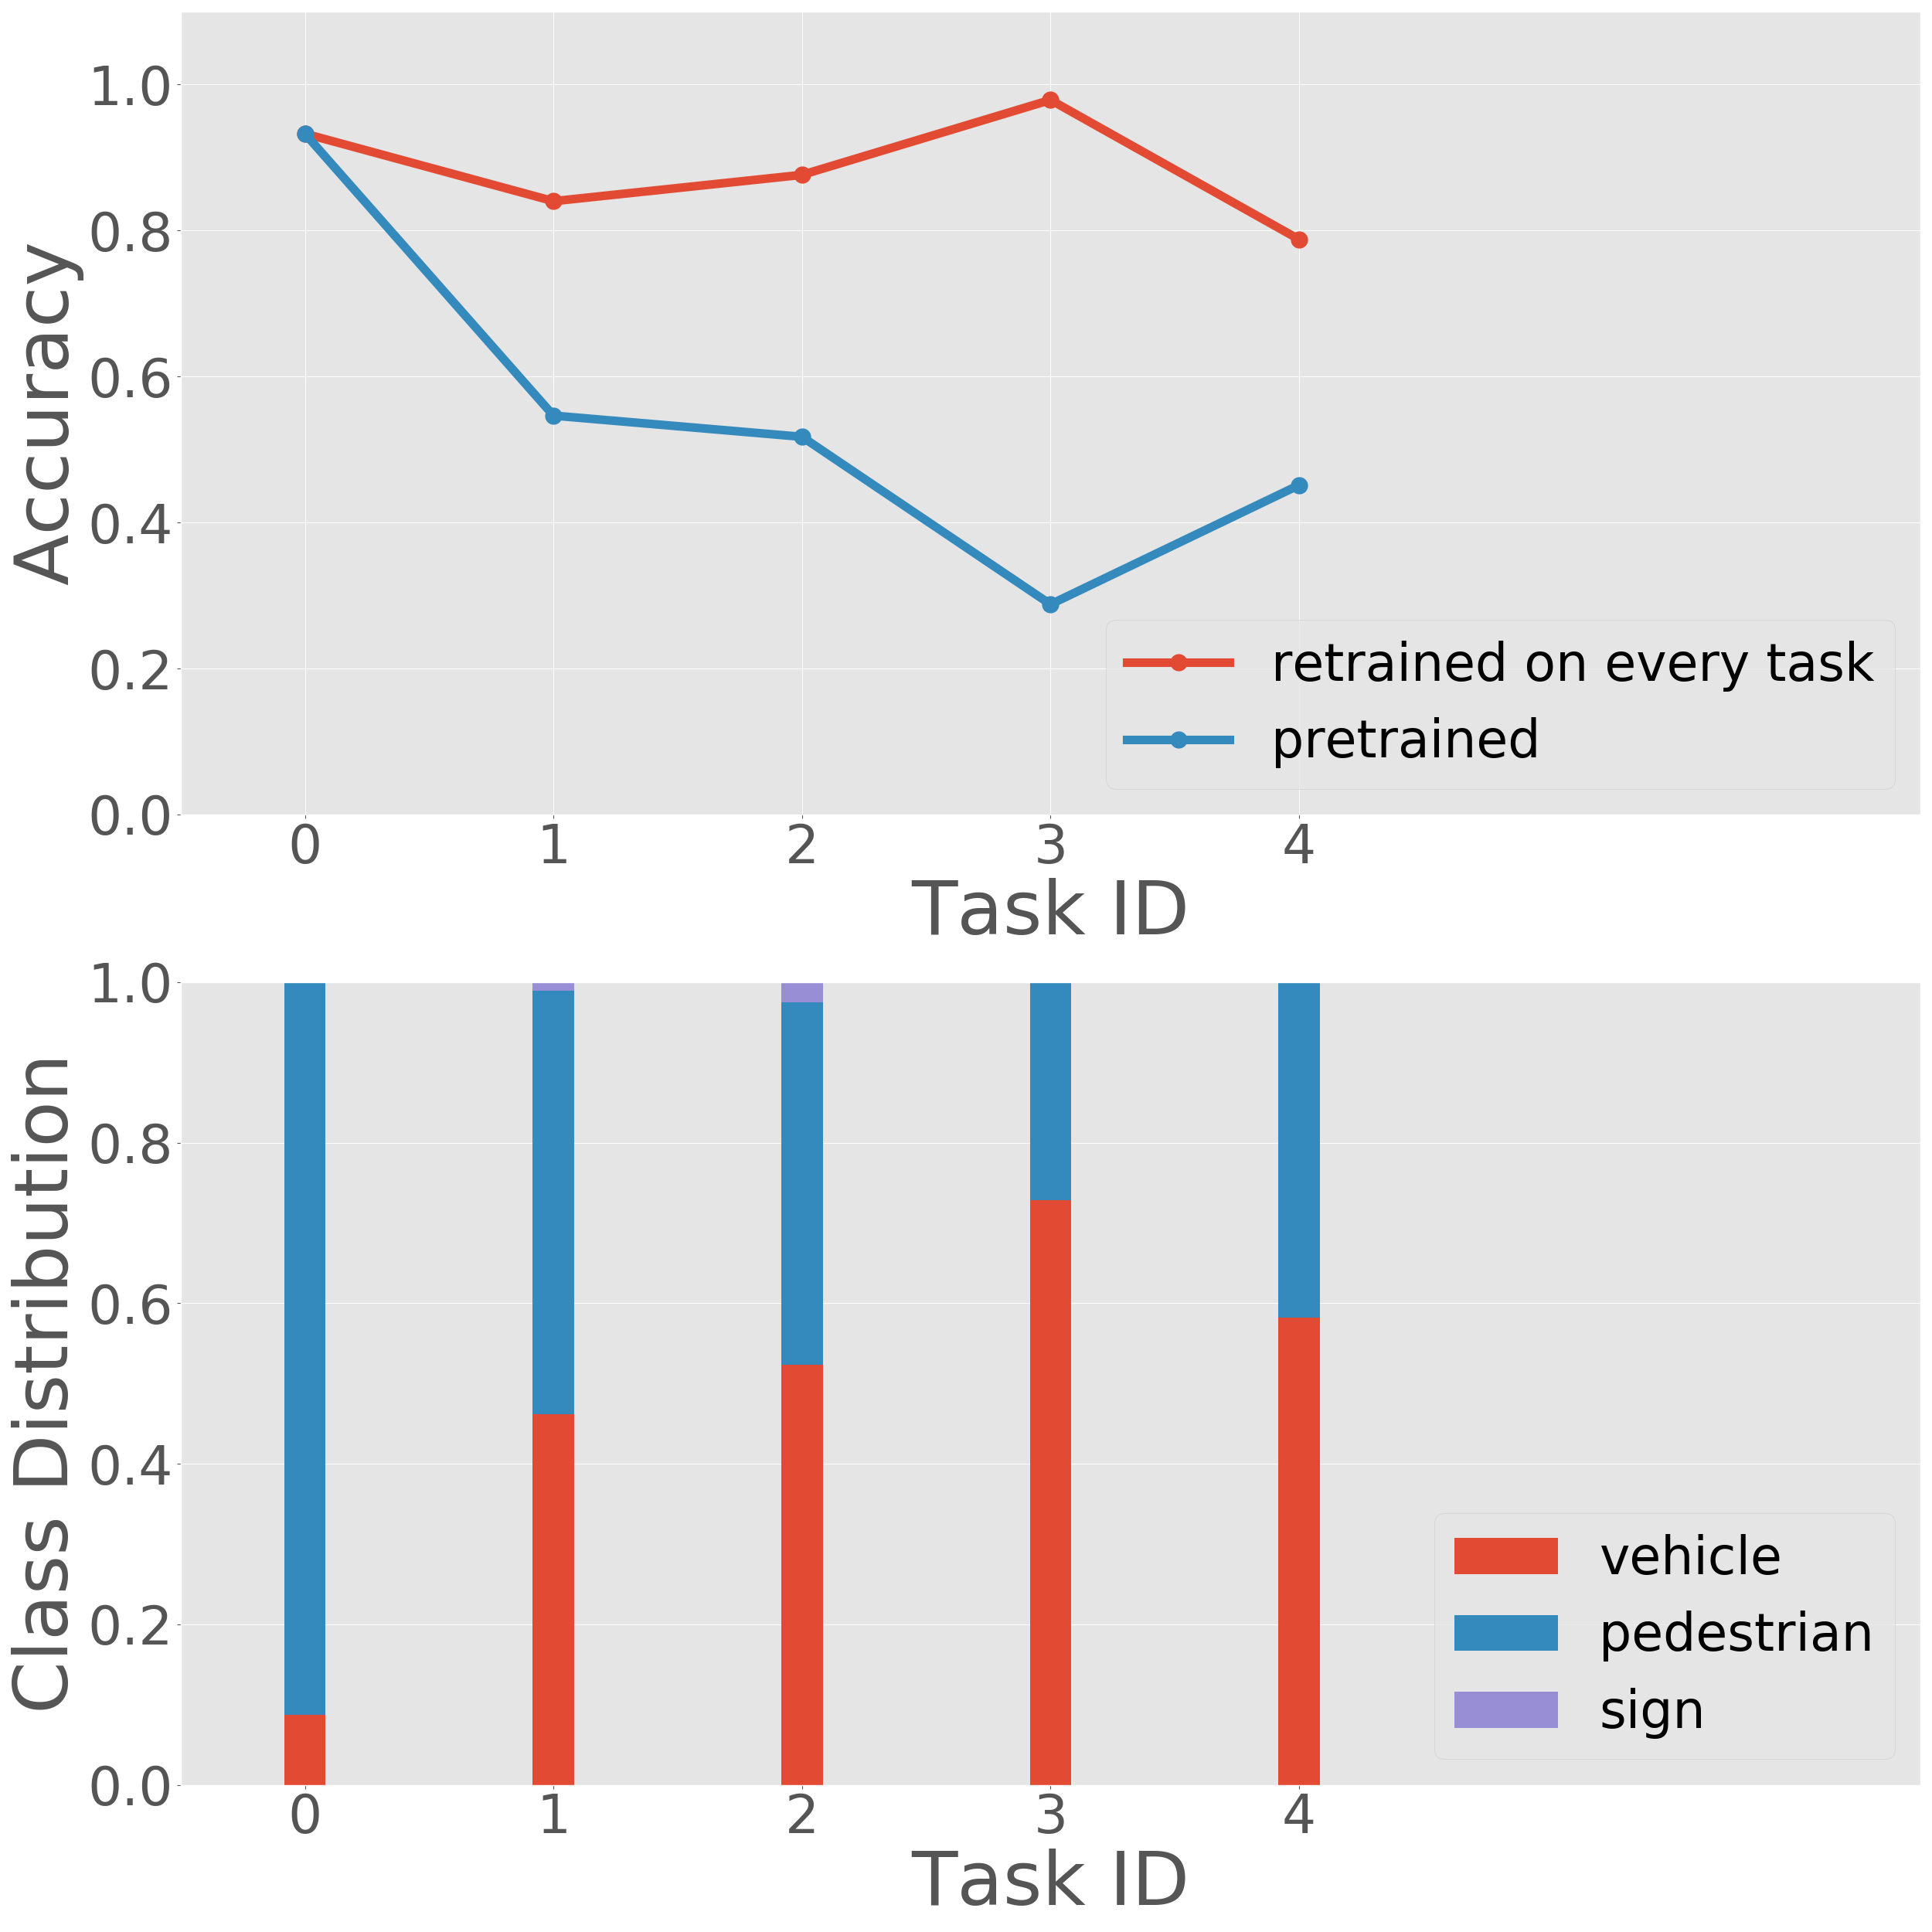
\includegraphics[width=\linewidth]{figures/motivation/Class_Incrementality/class_distribution_change_sf_27.png}
%     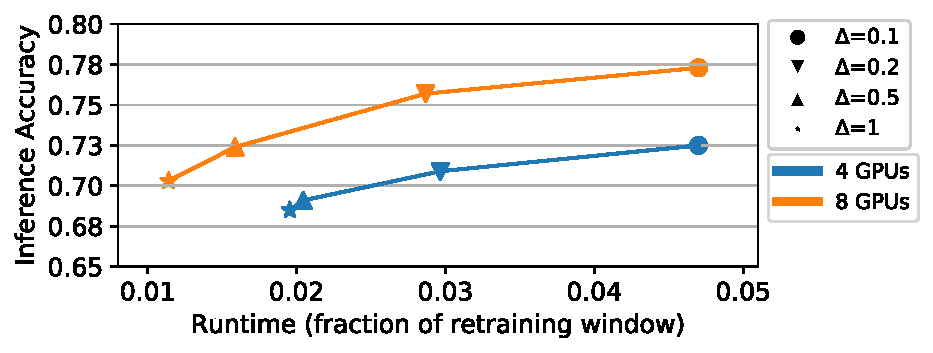
\includegraphics[width=\linewidth]{results/sensitivity/sensitivity_delta_acc_runtime_cityscapes_48gpu.pdf}
%      \caption{Effect of stealing parameter $\delta$ on the thief scheduler.}
%     \label{fig:sensitivity-delta}
%   \end{subfigure}
%   \caption{\bf Sensitivity Analysis Results.}
%   \label{fig:sensitivity-group}
% \end{figure}

% sensitivity to granularity
\mypara{Sensitivity to scheduling granularity} \ga{Change $\delta$ to $\Delta$ in the graphs and text.}
Finally, we show the sensitivity of \name to the allocation quantum $\delta$ (Algorithm \ref{algo:thief_sched}), which controls the runtime of the scheduling algorithm on the one hand and the result of the resource allocation on the other.
Figure~\ref{fig:sensitivity-delta} illustrates this tradeoff with the same setting as Figure~\ref{fig:scalability-gpus} (10 video streams with 4 or 8 GPUs provisioned).
Between $\delta=0.1$ and 1.0, higher $\delta$ reduces the runtime of the scheduler by 4$\times$, but the accuracy gain is severely affected. 
One should pick a higher $\delta$ only when the scheduler is relatively slow compared to a retraining window; otherwise, a low value of $\delta$ (fine-grained scheduling) is preferable.

\begin{figure}
  \centering
  \begin{subfigure}[t]{\linewidth}
    \centering
    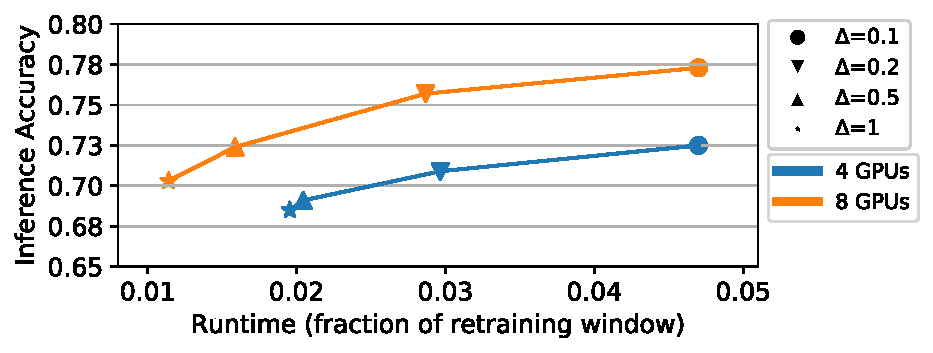
\includegraphics[width=\linewidth]{results/sensitivity/sensitivity_delta_acc_runtime_cityscapes_48gpu.pdf}
  \end{subfigure}
  \caption{\bf Effect of the $\delta$ parameter on the thief scheduler. Larger values decrease the accuracy but are faster to compute.}
  \label{fig:sensitivity-delta}
\end{figure}

\subsection{System Implementation}
\romil{WIP}
\romil{Move this up in the implementaiton section and start with this result.}
The Ekya implementation is an end-to-end system which can ingest video streams and distribute retraining and inference jobs over a pool of shared GPU resources. We ran this implementation on our Edge test-bed \ref{machine-specs}. The load on the system was varied by changing the number of video streams that must be processed in parallel on the same pool of resources. \cref{fig:sysimpl-result} illustrates the performance of Ekya comapred against the fair scheduler for Cityscapes and Waymo datasets. Ekya offers a consistently higher accuracy than the fair baseline (by upto 8\% points) and Ekya can achieve the same accuracy as the fair scheduler, but support $2\times$ the number of video streams in parallel on the same set of resources.

Ekya's performance is affected by the runtime efficiency of it's scheduler. The thief scheduler's search over the resource-configuration space \ref{algo:thief_sched} can be computationally expensive, but relative to retraining window size, it is a small cost. As shown in \Cref{fig:sensitivity-schedlatency}, the t  hief scheduler computes a resource allocation for a retraining window of 200 seconds even when multiple GPUs must be allocated.

\begin{figure}
  \centering
  \begin{subfigure}[t]{\linewidth}
    \centering
    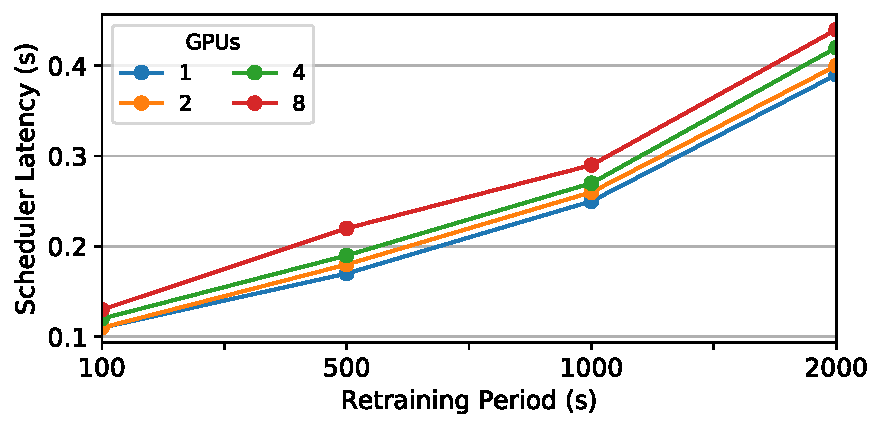
\includegraphics[width=\linewidth]{results/sensitivity/scheduler_resourcetime.pdf}
  \end{subfigure}
  \caption{\bf Thief scheduler latency for scheduling 10 video streams with varying available resource quantities and retraining period durations. The scheduler latency is a tiny fraction compared to the duration of the retraining period.  }
  \label{fig:sensitivity-schedlatency}
\end{figure}


\begin{figure}
  \centering
  \begin{subfigure}[t]{0.5\linewidth}
    \centering
    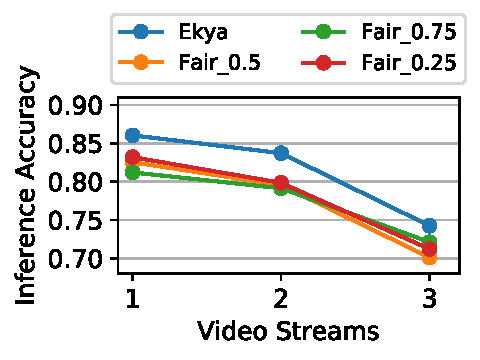
\includegraphics[width=\linewidth]{results/sys_impl/multicam_acc_vs_res_sysimpl_cityscapes.pdf} 
    \caption{Cityscapes}
    \label{fig:sysimpl-result-cityscapes}
  \end{subfigure}
  ~~~
  \begin{subfigure}[t]{0.5\linewidth}
    \centering
    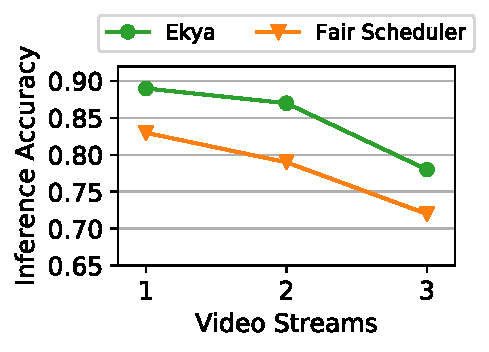
\includegraphics[width=\linewidth]{results/sys_impl/sysimpl_varyingcities_waymo.pdf} 
    \caption{Waymo}
    \label{fig:sysimpl-result-waymo}
  \end{subfigure}
  \caption{\bf End-to-end accuracy on the system implementation on 1 GPU with varying number of cities.}
  \label{fig:sysimpl-result}
\end{figure}